\documentclass[journal]{IEEEtran}

% ── Encoding ─────────────────────────────────────────────────
\usepackage[utf8]{inputenc}
\usepackage[T1]{fontenc}

% ── Math ─────────────────────────────────────────────────────
\usepackage{amsmath}
\usepackage{amssymb}
\usepackage{amsfonts}
\usepackage{amsthm}

% ── Tables ───────────────────────────────────────────────────
\usepackage{booktabs}
\usepackage{array}
\usepackage{multirow}
\usepackage{tabularx}
\usepackage{makecell}

% ── Graphics ─────────────────────────────────────────────────
\usepackage{graphicx}

% ── Misc ─────────────────────────────────────────────────────
\usepackage{xcolor}
\usepackage{enumitem}
\usepackage{caption}
\captionsetup{compatibility=false}
\usepackage{pifont}
\newcommand{\cmark}{\ding{51}}
\newcommand{\xmark}{\ding{55}}

% ── Algorithms ────────────────────────────────────────────────
\usepackage{algorithm}
\usepackage{algpseudocode}
\usepackage{stfloats}
\usepackage{url}

% ── Pipeline figure ───────────────────────────────────────────
\usepackage{tikz}
\usetikzlibrary{arrows.meta,positioning,fit,backgrounds}
\pgfdeclarelayer{background}
\pgfsetlayers{background,main}

% ── Citations (bibtex + IEEEtran.bst, see references.bib) ────
\usepackage{cite}

% ── Hyperref (loaded last so it wraps the packages above) ────
\usepackage[hidelinks]{hyperref}
\hypersetup{
  colorlinks = true,
  linkcolor  = blue,
  urlcolor   = blue,
  citecolor  = blue
}

% ── Theorem environments ──────────────────────────────────────
\newtheorem{theorem}{Theorem}
\newtheorem{proposition}{Proposition}
\newtheorem{definition}{Definition}
\newtheorem{corollary}{Corollary}
\newtheorem{lemma}{Lemma}
\newtheorem{remark}{Remark}

% -------------------------------------------------------------------------
% DRAFT v2 — Risk-Aware Quantum DRL for BBR-v3 over Starlink
% Status: system-design proposal draft (pre-experiment).
% Author names/affiliations to be filled in.
% -------------------------------------------------------------------------

\begin{document}

\title{Risk-Aware Quantum Deep Reinforcement Learning for Adaptive BBR-v3
Pacing over Starlink LEO Networks: A System Design}

\author{Tien~Nguyen,~\IEEEmembership{}% TODO: full author list + affiliations
\thanks{Draft v2: internal design document. Not for distribution.}}

\maketitle

\begin{abstract}
% TODO: write after the full paper is finalized.
\end{abstract}

\begin{IEEEkeywords}
BBR-v3, congestion control, Starlink, LEO satellites, quantum machine
learning, reinforcement learning, alpha-fairness.
\end{IEEEkeywords}

% =========================================================================
\section{Introduction}
% =========================================================================
\IEEEPARstart{L}{ow} Earth Orbit (LEO) mega-constellations have transformed
satellite internet from supplemental backhaul into a mainstream access
technology. SpaceX's Starlink, the most mature deployment, serves millions of
subscribers through phased-array user links, Ka-band feeder links, and laser
inter-satellite links (ISLs)~\cite{desilva2026tmc}. However, LEO-specific
dynamics, including periodic handovers on a $\sim$15\,s cycle, atmospheric
attenuation, ISL disruptions, and RTTs ranging from $\sim$47\,ms to over
370\,ms depending on the terrestrial endpoint, create non-stationary path
conditions that challenge transport-layer control loops.

Google's BBR-v3 explicitly models bottleneck bandwidth and propagation delay,
and a recent global six-city experimental study~\cite{desilva2026tmc,
desilva2026icoin} demonstrated that BBR-v3 achieves multiplicative throughput
gains over Cubic, Vegas, and Hybla on Starlink. Yet the same study revealed a
consistent cost: elevated retransmissions caused by BBR's aggressive probing,
which applies \emph{fixed, environment-agnostic} gain factors regardless of
imminent handovers or degraded link conditions. The study's own analytical
contribution: closed-form failure probabilities for atmospheric, ISL, and
handover events, combined into an end-to-end loss probability
$p^{\mathrm{tot}}$, together with a fluid model of BBR-v3 dynamics and an
M/G/1 queuing approximation, explains these observations but has not yet
been used to \emph{control} the protocol.

This design closes that loop. We ask: \emph{can a lightweight learning agent,
informed by predictive risk signals, adapt BBR-v3's pacing gain to retain its
throughput advantage while reducing retransmissions and preserving fairness
toward competing flows?} Three constraints shape the answer. First, the agent
must be small enough for per-decision-interval inference on an end host.
Second, fairness must be a first-class objective: linear reward functions of
the form $\alpha\cdot\mathrm{throughput}-\beta\cdot\mathrm{delay}$ are known
to drift with bandwidth and delay conditions~\cite{yu2026dnccq}, which is
untenable when RTT varies by $8\times$ across paths. Third, training cannot
rely on naive trace replay: traces collected under stock BBR-v3 contain no
information about counterfactual actions, so an explicit environment model is
required.

Our contributions are as follows:
\begin{itemize}
  \item \textbf{Risk-aware state design:} A six-dimensional state combining
  BBR internals ($\hat{B}_\theta$, inflight/BDP), live telemetry (RTT ratio,
  M/G/1 queue estimate), and two closed-form risk features
  ($p^{\mathrm{tot}}$ and handover ETA $\Delta T_{\mathrm{ho}}$ from TLE and
  weather proxies), enabling the agent to act \emph{before} predictable
  failures.
  \item \textbf{Compact quantum actor--critic:} A six-qubit quantum advantage
  actor--critic (QA2C) with angle encoding and a hardware-efficient
  ansatz, totaling 36--54 quantum parameters, paired with an
  identically-budgeted classical baseline to isolate the quantum
  contribution.
  \item \textbf{$\alpha$-fair logarithmic reward:} A reward built on the
  $\alpha$-fair utility family, whose $\alpha{=}1$ instance embeds
  proportional fairness into the objective by the network utility
  maximization equivalence~\cite{kelly1998, mo2000}, with a loss-\emph{change}
  penalty robust to Starlink's non-congestive baseline loss.
  \item \textbf{Trace-calibrated model-based training:} An offline training
  environment built from the base study's fluid model and M/G/1
  approximation, calibrated per location from six-city traces, reserving the
  physical testbed for sim-to-real evaluation with deployment guardrails.
\end{itemize}

The remainder of this draft is organized as follows.
Section~\ref{sec:related} positions this design against prior work and
states the research questions that follow from the identified gap.
Section~\ref{sec:design}
details the system architecture. Section~\ref{sec:training} presents the
training methodology. Section~\ref{sec:eval} defines the evaluation
protocol. Section~\ref{sec:conclusion} concludes.

% =========================================================================
\section{Related Work and Research Questions}
\label{sec:related}
% =========================================================================

\subsection{BBR-v3 over Starlink: Established Findings and the Open Gap}
\label{sec:gap}
The six-city experimental studies that this work builds
upon~\cite{desilva2026tmc, desilva2026icoin} established three findings.
First, BBR-v3 consistently dominates Cubic, Vegas, and Hybla in both
dedicated and competitive streams over Starlink, with median downlink
throughput exceeding 100\,Mbps at every location. Second, this dominance
carries a systematic cost: retransmission inflation driven by aggressive
bandwidth probing, most pronounced on high-RTT paths, a direct consequence
of gain factors that remain \emph{fixed and environment-agnostic} even when
a handover is seconds away or atmospheric conditions degrade the link.
Third, the studies contributed analytical machinery: closed-form failure
probabilities for atmospheric, ISL, and handover events composing an
end-to-end loss probability $p^{\mathrm{tot}}$, a fluid model of BBR-v3
state dynamics, and an M/G/1 queuing approximation, used, however, only to
\emph{explain} the measurements.

The research gap follows from the base studies' own conclusions, which
identify the adaptation of BBR parameters to satellite characteristics and
the balancing of throughput against retransmission efficiency as the open
problem, alongside fairness and coexistence assessment deferred to future
work~\cite{desilva2026tmc, desilva2026icoin}. Concretely, the gap has three
components: (i)~BBR-v3's probing parameters are static despite predictable
LEO impairments; (ii)~the analytical models exist but have never been placed
\emph{in the control loop}; and (iii)~fairness toward competing flows
remains unevaluated. The present design addresses all three: a learning
agent adapts \texttt{pacing\_gain} online, the analytical models become both
state inputs (risk features) and the training environment, and an
$\alpha$-fair objective makes coexistence a first-class design property.

\subsection{Learning-Based Congestion Control}
Measured against this gap, existing learning-based approaches fall short on
at least one component. Offline-learned schemes such as RemyCC and Indigo
generalize poorly beyond their training conditions. Online DRL
approaches (Aurora~\cite{aurora}, MVFST-RL, Sage, Astraea) adapt at
runtime but \emph{replace} the congestion controller wholesale rather than
augmenting BBR's model-based machinery, employ fixed or RTT-proportional
sampling, and rely on linear rewards that drift with bandwidth and delay
conditions~\cite{yu2026dnccq}, untenable on paths whose RTT spans
47--370+\,ms. None incorporates predictive link-risk information.
DNCCQ-PPO~\cite{yu2026dnccq} resolves the sampling and reward-drift issues
for XQUIC via a piecewise \emph{minRTT-100} interval and a logarithmic
reward, reporting faster convergence and up to 69.6\% latency reduction
versus CUBIC in satellite simulation; we adopt both mechanisms. However,
DNCCQ-PPO likewise substitutes the controller, is evaluated on emulated
constellations rather than a production LEO network, and its fairness
treatment remains empirical rather than embedded in the objective. Outside
RL, Copa's~\cite{copa} objective
$\log(\mathrm{tput})-\delta\log(\mathrm{delay})$ independently evidences the
soundness of logarithmic utilities in congestion control, and
Orca~\cite{orca} validates the hybrid pattern (learning layered on a
classical controller) that we instantiate with BBR-v3.

\subsection{Quantum Reinforcement Learning}
Variational quantum circuits have been formulated as actor--critic agents in
the quantum advantage actor--critic (QA2C) framework, and
quantum self-attention architectures (QASA) extend the toolkit; since VQCs
are architecturally equivalent to quantum neural networks, these frameworks
require no bespoke blocks. To our knowledge, no prior work applies quantum
RL to transport-layer congestion control and, more importantly for
rigor, published QRL studies rarely control for parameter count against
classical baselines. We therefore treat the quantum core as a hypothesis to
be tested (RQ4) rather than an assumed advantage.

\subsection{Research Questions}
\label{sec:rq}
The gap established above motivates four research questions.
\textbf{RQ1:} Does risk-aware adaptive gain reduce retransmissions while
retaining BBR-v3's throughput advantage in isolation?
\textbf{RQ2:} Does the learned policy improve $\alpha$-fair coexistence with
competing CCAs?
\textbf{RQ3:} Do the risk features ($s_5,s_6$) contribute measurably beyond
telemetry alone?
\textbf{RQ4:} Does the quantum core outperform, match, or trail a
classical network of equal parameter budget?

% =========================================================================
\section{System Design}
\label{sec:design}
% =========================================================================

\subsection{Architecture Overview}
The pipeline comprises five stages, illustrated in
Fig.~\ref{fig:pipeline}: (1)~data sources, (2)~state construction,
(3)~quantum encoding, (4)~a quantum actor--critic core, and (5)~action and
learning signal. A governing design principle separates the roles of
statistics and learning: \emph{risk estimation is closed-form statistics,
not machine learning}. The learning happens downstream, in how the agent
acts on those signals. An offline training loop
(Section~\ref{sec:training}) wraps Stages 2--5; online deployment executes
forward passes only, under the guardrails of
Section~\ref{sec:guardrails}.

\begin{figure*}[!t]
\centering
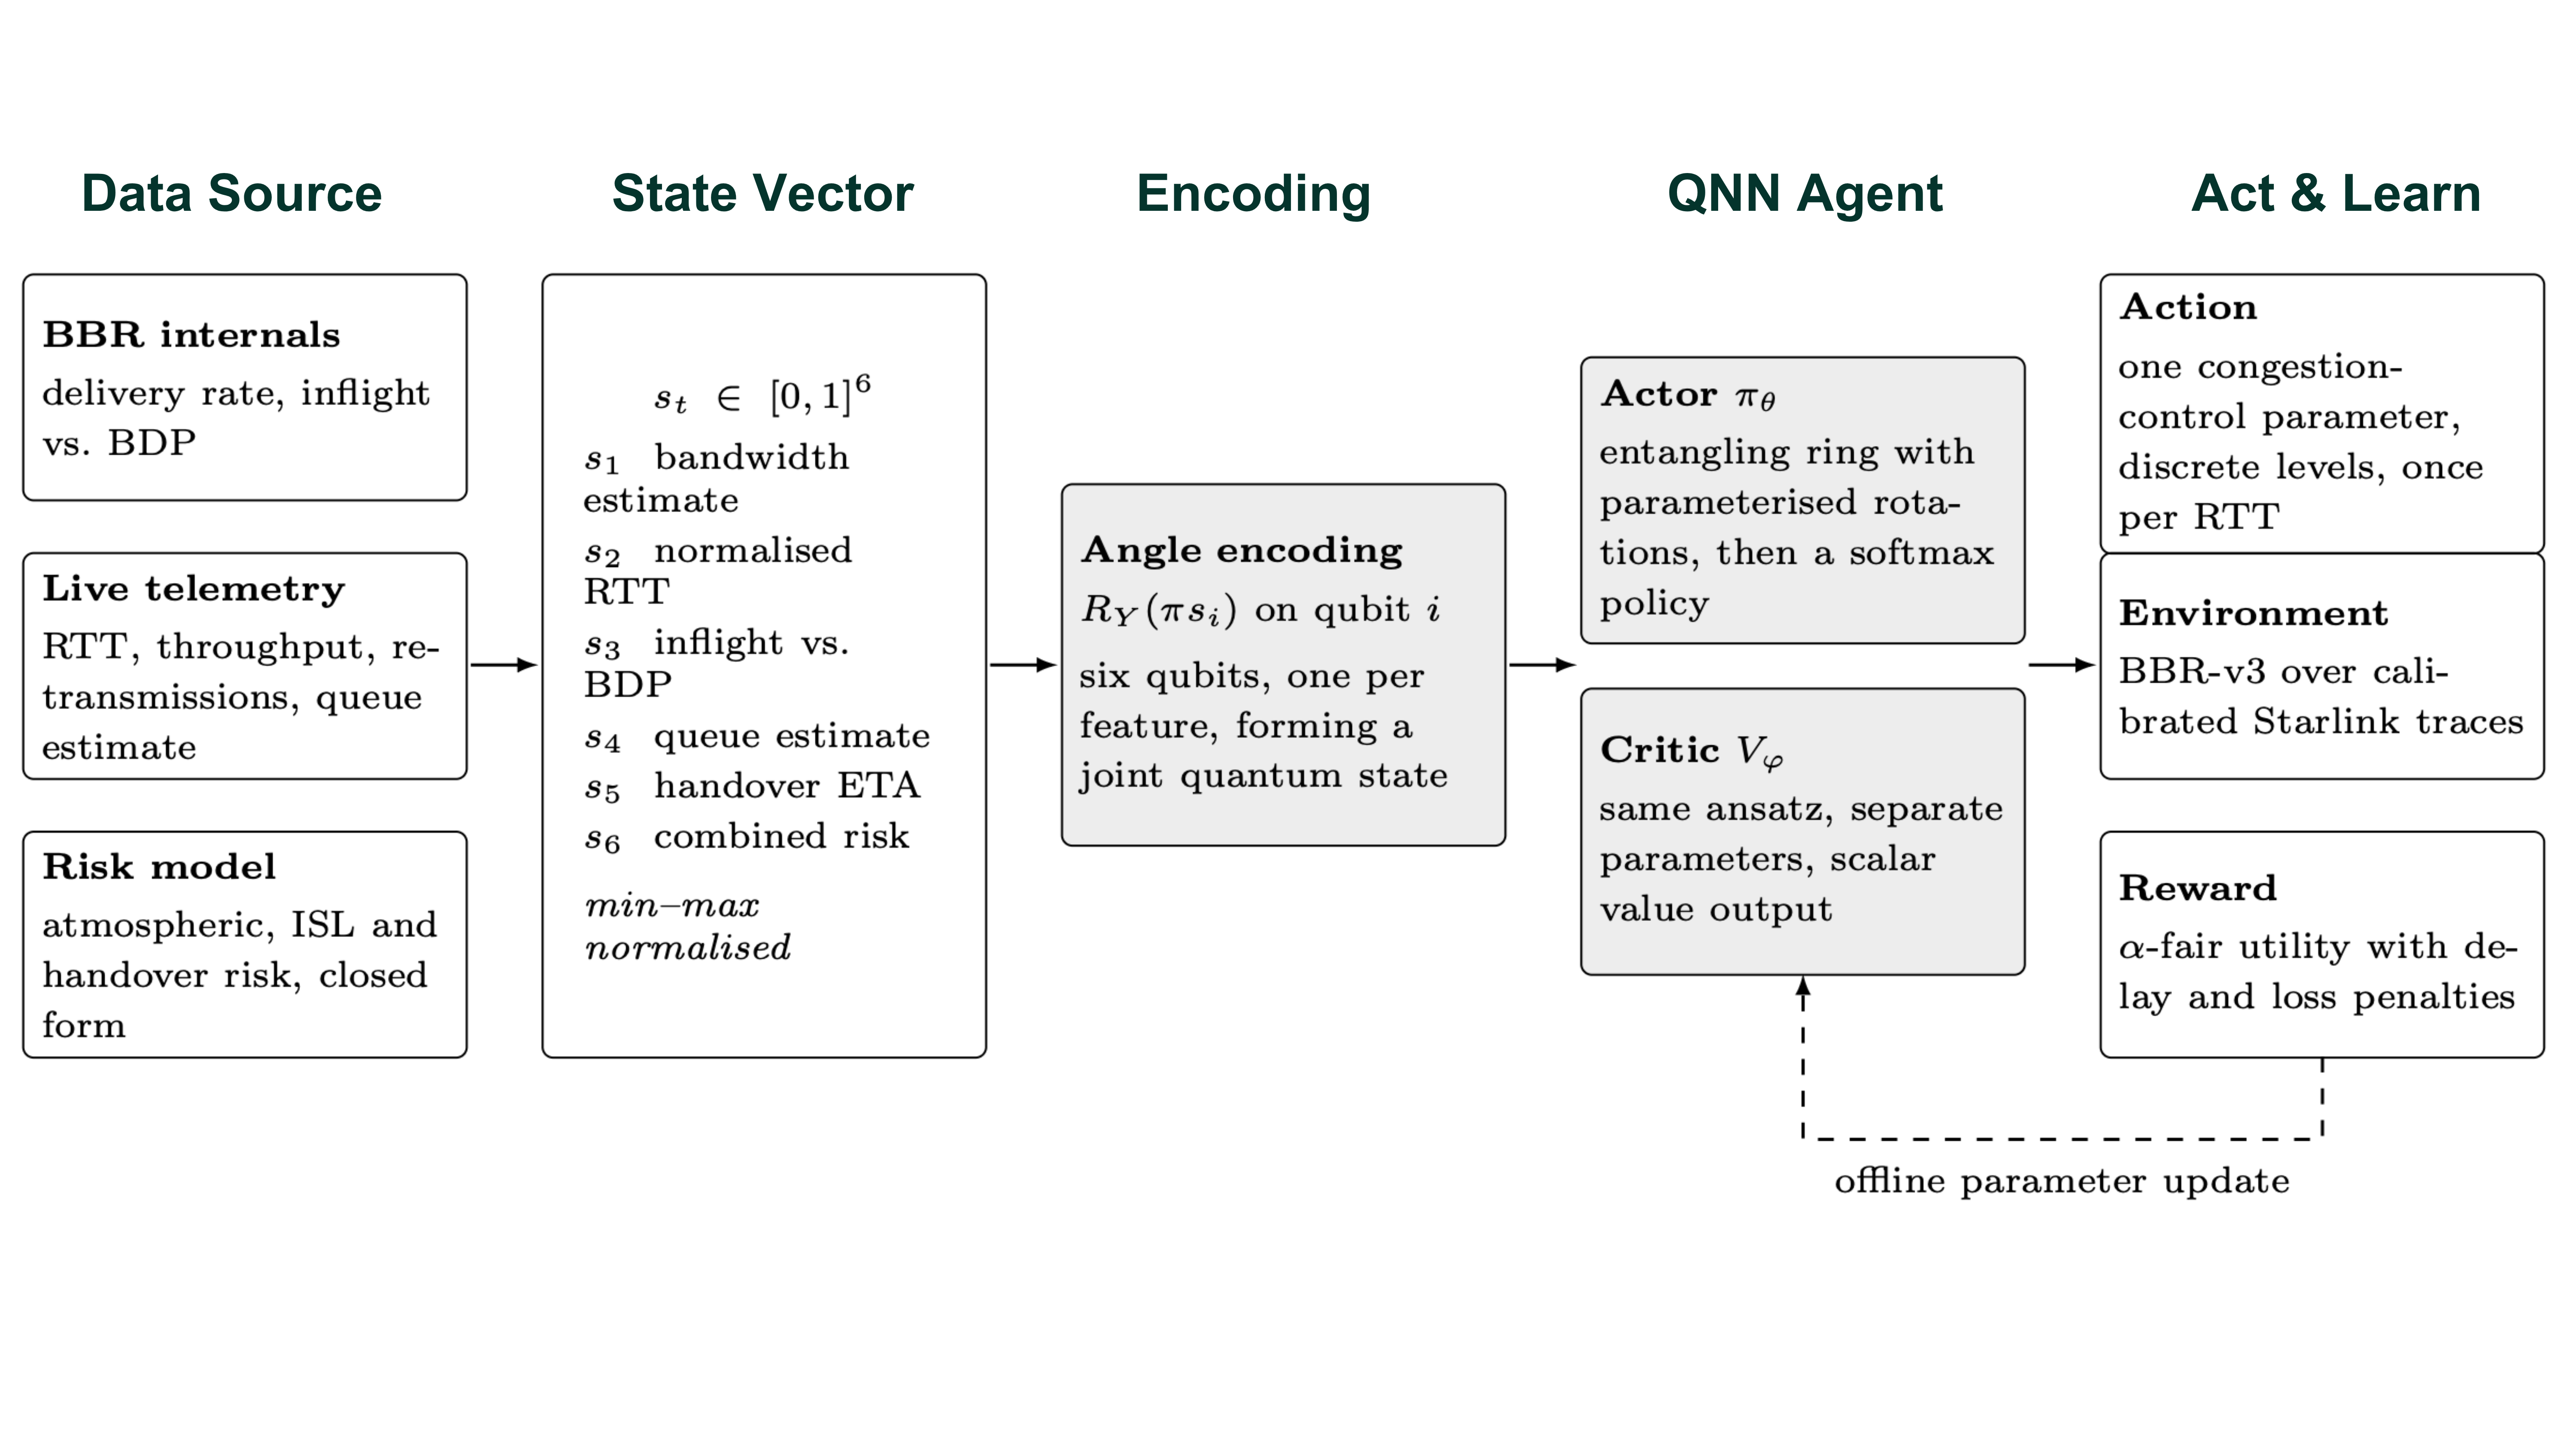
\includegraphics[width=\textwidth]{figures/pipeline1.png}
\caption{System pipeline. Three data sources (BBR internals, live
telemetry, closed-form risk) are assembled into a six-dimensional state
vector, angle-encoded onto six qubits, and processed by the quantum
actor--critic core to select a \texttt{pacing\_gain} action applied to
BBR-v3. The resulting reward closes an offline training loop (dashed
arrow) back to the critic; online deployment uses the trained actor only.}
\label{fig:pipeline}
\end{figure*}

\subsection{Stage 1: Data Sources (Three Origins, Six
Features)}
\label{sec:state}
Six features are drawn from three origins:
\begin{itemize}
  \item \emph{BBR internals} (2): bottleneck bandwidth estimate
  $\hat{B}_\theta$ from windowed-max filtering of delivery-rate samples
  (kernel \texttt{tcp\_sock}), and inflight volume $v_t$ relative to
  estimated BDP. These anchor the state in the protocol's own path model.
  \item \emph{Live telemetry} (2): per-interval RTT (as
  $\mathrm{RTT}_t/\mathrm{RTT}_{\min}$) from \texttt{iperf3}; queue
  occupancy $q_t$ estimated via the base study's M/G/1 approximation
  (Eqs.~30--32 of~\cite{desilva2026tmc}).
  \item \emph{Risk model} (2): the closed-form physics of the base
  study: atmospheric (Eq.~9), ISL (Eq.~15), and handover (Eq.~19) failure
  probabilities composed into the end-to-end $p^{\mathrm{tot}}$
  (Eqs.~20--21), and the handover ETA $\Delta T_{\mathrm{ho}}$ estimated
  from TLE ephemerides and elevation geometry.
\end{itemize}
\emph{Sourcing caveat:} ISL and handover terms are not exposed by
Starlink's public API; $p^{\mathrm{tot}}$ and $\Delta T_{\mathrm{ho}}$ are
therefore proxies computed from TLE and weather data, and their empirical
validity is tested \emph{before} training (Section~\ref{sec:riskval}).

\subsection{Stage 2: State Vector and Normalization}
The state $s_t\in[0,1]^6$ is deliberately balanced (two features per
origin) so the agent observes protocol state and environmental risk
jointly; $s_5$ and $s_6$ are what make the design \emph{risk-aware},
allowing action before a predictable failure. Min--max normalization is
required by angle encoding (rotation angles must lie in a fixed range), and
dimensionality is capped at six because barren-plateau risk grows with
register width. Table~\ref{tab:norm} specifies each mapping; the listed
constants derive from the base study's measurements and are re-estimated
from the training dataset (per-location 99th percentiles) rather than
hard-coded.

\begin{table}[!t]
\caption{State Features and Normalization to $[0,1]$}
\label{tab:norm}
\centering
\footnotesize
\begin{tabularx}{\columnwidth}{@{}llX@{}}
\toprule
Feature & Mapping & Constants / rationale \\
\midrule
$s_1$: $\hat{B}_\theta$ & $\hat{B}_\theta / B_{\max}$ &
  $B_{\max}\!\approx\!350$\,Mbps (Sydney downlink) \\
$s_2$: RTT ratio &
  $\frac{\mathrm{RTT}_t-\mathrm{RTT}_{\min}}{\mathrm{RTT}_{\max}-\mathrm{RTT}_{\min}}$ &
  47\,ms (Sydney)--$\sim$400\,ms (S\~{a}o Paulo) \\
$s_3$: $v_t/\mathrm{BDP}$ & clip by $/2.5$ &
  $>\!1$ = queue buildup; 2.5 covers $5/4$ probe \\
$s_4$: $q_t$ & $q_t / q_{\mathrm{cap}}$ &
  $q_{\mathrm{cap}}=50$ pkts (saturation cap) \\
$s_5$: $\Delta T_{\mathrm{ho}}$ &
  $1-\Delta T_{\mathrm{ho}}/T_{\mathrm{orbit}}$ &
  inverted: higher = more urgent; $T_{\mathrm{orbit}}\!\approx\!5.4$\,min \\
$s_6$: $p^{\mathrm{tot}}$ & identity &
  already a probability in $[0,1]$ \\
\bottomrule
\end{tabularx}
\end{table}

\subsection{Stage 3: Quantum Encoding}
Each feature is angle-encoded as $R_Y(\pi s_i)$ on qubit~$i$ (one shallow
gate per feature), so the six qubits form a single joint quantum state
$|\psi(s_t)\rangle\in\mathbb{C}^{64}$ in which downstream entangling layers
can capture correlations between network signals and risk. Amplitude
encoding was rejected: it requires deep state-preparation circuits and
complicates gradients, a poor fit for six features.

\subsection{Stage 4: QNN Actor--Critic Core}
Two separate QNNs (actor $\pi_\theta$ and critic $V_\phi$) share an
identical architecture with independent weights. The variational block
repeats $L\in\{2,3\}$ times: a CNOT entangling ring
($q_i{\to}q_{i+1}$, wrapped) followed by $R_Z R_Y R_Z$ rotations per qubit,
yielding $6\times 3\times L=18L=36$--$54$ quantum parameters. The actor
maps per-qubit expectations $\langle Z_i\rangle$ through a $6{\times}5$
linear head and softmax to a policy over five gain levels; the critic maps
$\sum_i\langle Z_i\rangle$ through a linear head to a scalar value. The
design follows the QA2C framework; since variational
quantum circuits are architecturally equivalent to quantum neural networks,
no additional block is introduced. If $L\le 3$ underfits, capacity is added
via data re-uploading (re-encoding $s_t$ between variational layers) rather
than widening the register.

\emph{Gradients:} On the simulator we use analytic backpropagation
(PennyLane \texttt{default.qubit}); the parameter-shift rule is retained
only as the hardware-compatible path, as it requires two circuit
evaluations per parameter per gradient.

\emph{Classical baseline:} A multilayer-perceptron actor--critic with an
identical $\sim$36--54 parameter budget is trained under identical state,
action, reward, environment, and seeding, to isolate the quantum
contribution (RQ4).

\subsection{Stage 5: Action, Decision Interval, and Learning
Signal}
\label{sec:reward}

\subsubsection{Action Space and Protocol Hook}
Following supervisor guidance to begin with a single parameter group, the
agent controls only
$\texttt{pacing\_gain}\in\{0.75, 0.9, 1.0, 1.1, 1.25\}$. BBR-v3's ProbeBW
phase cycles through UP $\to$ DOWN $\to$ CRUISE $\to$ REFILL; the agent
overrides the default gain (1.0) at the start of each ProbeBW\_CRUISE
sub-state only, leaving all other states (including the probing gains of
UP/DOWN) stock. The kernel hook is \texttt{bbr2\_set\_pacing\_rate()},
verified against the IETF BBR draft~\cite{ietfbbr}. Extension to
\texttt{inflight\_hi/lo} and early ProbeRTT triggering is deferred to later
phases.

\subsubsection{Decision Interval}
Because path RTTs span 47--370+\,ms across locations, a fixed once-per-RTT
interval would skew the effective horizon of the discount factor by
$\sim$8$\times$. We therefore adopt the minRTT-100 rule~\cite{yu2026dnccq}:
\begin{equation}
T_{\mathrm{dec}} =
\begin{cases}
2\cdot \mathrm{minRTT}, & \mathrm{minRTT}\le 100\,\mathrm{ms},\\
100\,\mathrm{ms} + \mathrm{minRTT}, & \text{otherwise}.
\end{cases}
\end{equation}

\subsubsection{Reward and Fairness: Re-Framing the Learning Signal}
An earlier iteration of this design used a linear reward,
$r_t = w_1\,\mathrm{tput}_t/\hat{B}_\theta - w_2\,\mathrm{rtx}_t -
w_3\max(0, q_t-q_{\mathrm{tgt}})$, with Jain's index measured post hoc
under competing flows. Two deficiencies motivate its replacement. First,
linear rewards drift with bandwidth and delay
conditions~\cite{yu2026dnccq}: the policy optimum shifts across paths whose
capacity and RTT differ by an order of magnitude. Second, treating fairness
as an externally measured index leaves the objective itself
fairness-blind, and Jain's index in particular captures only dispersion,
not any principled allocation target. We therefore re-frame both at once:
\begin{equation}
r_t \;=\; U_\alpha(x_t) \;-\; \delta\,
\log\!\frac{\mathrm{RTT}_t}{\mathrm{RTT}_{\min}} \;-\; \beta\, l_t,
\label{eq:reward}
\end{equation}
where $x_t$ is the delivered throughput in the decision window,
\begin{equation}
U_\alpha(x)=
\begin{cases}
\dfrac{(x+\varepsilon)^{1-\alpha}}{1-\alpha}, & \alpha\neq 1,\\[6pt]
\log(x+\varepsilon), & \alpha=1,
\end{cases}
\qquad
l_t=\frac{\mathrm{rtx}_t-\mathrm{rtx}_{t-1}}{\mathrm{rtx}_{t-1}+\varepsilon}.
\end{equation}
Each term has an explicit network origin: $x_t$ from delivery-rate (ACK)
sampling, the RTT ratio from sender-side measurement, and $l_t$ from
retransmission counters across consecutive windows. Three properties
motivate this form. (i)~\emph{Scale invariance:} the logarithm renders the
utility consistent across 50--350\,Mbps paths without per-location reward
normalization. (ii)~\emph{Fairness by construction:} per-flow logarithmic
utility maximization yields proportionally fair
equilibria~\cite{kelly1998, mo2000}; $\alpha$ generalizes this to the full
fairness spectrum ($\alpha{=}0$ throughput-max, $\alpha{=}1$ proportional,
$\alpha{\to}\infty$ max--min). Fairness thus moves from a measured
afterthought into the objective itself. Jain's index is dropped from this
design entirely rather than retained as a secondary metric: it scores any
equal-throughput split as maximally fair irrespective of path RTT or
capacity, which is precisely the allocation notion this reward is designed
to move \emph{away} from. Reporting it would reintroduce the train/eval
mismatch that motivated re-framing the reward in the first place. Evaluation
instead reuses the same $U_\alpha$ family as a post-hoc metric
(Section~\ref{sec:eval}). (iii)~\emph{Robustness to baseline loss:}
penalizing the loss \emph{change rate} rather than absolute loss prevents
the agent from conflating Starlink's non-congestive losses (handover,
atmospheric) with congestion, the very confusion BBR was designed to
avoid.

One design invariant is preserved from the earlier iteration: \emph{risk
lives in the state, not the reward}. The reward remains outcome-only
(throughput, delay, loss trend); $s_5$ and $s_6$ inform the policy's
anticipation but are never rewarded directly, avoiding incentive to game
the risk estimates. We set $\varepsilon=10^{-6}$ (throughput is genuinely
zero during handover gaps) and initialize $(\delta,\beta)=(1.0,0.5)$
per~\cite{yu2026dnccq}, subject to grid search; $\alpha{=}1$ is the MVP
setting, swept in ablation.

% =========================================================================
\section{Training Methodology}
\label{sec:training}
% =========================================================================

\subsection{Why Naive Trace Replay Fails}
The available traces were collected under stock BBR-v3 with default gains.
A2C is on-policy, and the traces contain no counterfactual information about
how the network responds to non-default gains: action coverage is
effectively zero. Training directly on replayed traces would therefore learn
incorrect dynamics.

\subsection{Trace-Calibrated Fluid-Model Simulator}
\label{sec:sim}
We instead construct a Gym-style environment whose dynamics engine is the
base study's own analytical machinery: the BBR-v3 fluid model (pacing rate,
inflight evolution, cruise/drawdown indicators; Eqs.~22--29
of~\cite{desilva2026tmc}) with the agent's chosen gain substituted for the
default $5/4$--$3/4$ factors, coupled with the M/G/1 queuing approximation
(Eqs.~30--32) and the risk process $p^{\mathrm{tot}}(t)$ driving loss
events. Traces serve two roles only: \emph{calibration} of per-location
environment parameters (bandwidth process, base RTT distribution, queue
parameters, risk-model inputs) and \emph{validation}: replaying stock
BBR-v3 inside the simulator must reproduce the empirical distributions of
throughput, RTT, and retransmissions before any training run is accepted.
One episode corresponds to a 300\,s run (matching the base study's
measurement protocol); transitions occur every $T_{\mathrm{dec}}$; the
target is 200--500 episodes, augmented by domain randomization around
calibrated parameters for sim-to-real robustness. Should simulator fidelity
prove insufficient, the fallback is a DNCCQ-style emulation
architecture~\cite{yu2026dnccq} (Mininet with satellite delay/loss profiles,
message-middleware decoupling).

Methodologically, this converts the base study's models from
\emph{explanatory} artifacts into the \emph{training environment}, closing a
loop: model $\rightarrow$ environment $\rightarrow$ agent $\rightarrow$
same testbed.

\subsection{Risk-Feature Validation (Pre-Training Gate)}
\label{sec:riskval}
Before any training, the proxy validity of $s_5$ and $s_6$ is tested against
the traces: (i)~compute $\Delta T_{\mathrm{ho}}$ from TLE ephemerides for
the exact trace period and location; (ii)~run event-aligned
cross-correlation between predicted handover windows ($\sim$15\,s cycle) and
observed loss/RTT-spike events; (iii)~correlate $p^{\mathrm{tot}}$ against
loss rates using historical weather data. Strong correlation retains the
features as a core contribution; weak correlation demotes them to
ablation-only status and is itself a reportable finding on proxy validity.
This gate costs no training compute yet determines the value of half the
state vector.

\subsection{Deployment Guardrails}
\label{sec:guardrails}
Online operation is forward-pass only, with three safeguards: (i)~a
\emph{clamp} restricting overrides to ProbeBW\_CRUISE; (ii)~a
\emph{fallback} reverting to the default gain if retransmissions exceed a
threshold for $k{=}5$ consecutive intervals; (iii)~a measured
\emph{latency budget}: six-qubit inference reduces to $64$-dimensional
linear algebra and must satisfy $t_{\mathrm{inf}} < T_{\mathrm{dec}}/10$
(reference point: 2.1\,ms model latency in~\cite{yu2026dnccq}).

% =========================================================================
\section{Evaluation Protocol}
\label{sec:eval}
% =========================================================================

\subsection{Scenarios and Metrics}
\emph{Scenario A (isolation):} the agent-augmented BBR versus stock BBR-v3,
Cubic, Vegas, and Hybla run individually; metrics mirror the base study
(throughput, retransmissions, RTT variance) for direct comparability.
\emph{Scenario B (coexistence):} the agent runs concurrently with the four
CCAs over one Starlink link. Fairness and efficiency across the $n$
concurrently competing flows are measured with the same $\alpha$-fair family
as the reward, applied post hoc as a pure metric rather than a training
signal, and swept over $\alpha\in\{0,1,2,\infty\}$ to cover
throughput-maximizing, proportionally fair, and max--min regimes:
\begin{equation}
\Phi_\alpha(x) = \sum_{i=1}^{n} U_\alpha(x_i), \qquad
\rho_\alpha = \frac{\Phi_\alpha(x^{\mathrm{achieved}})}{\Phi_\alpha(x^\star)},
\label{eq:fairness}
\end{equation}
where $x=(x_1,\dots,x_n)$ is the vector of per-flow throughputs measured over
the evaluation window (distinct from the single-flow, per-decision-interval
$x_t$ of Eq.~\ref{eq:reward}), and $x^\star$ is the $\alpha$-fair-optimal
allocation for the same measured aggregate capacity, obtained by solving
$\max_x \Phi_\alpha(x)$ subject to that capacity constraint (a convex
program, with closed-form water-filling at $\alpha\to\infty$). The
efficiency ratio $\rho_\alpha\in(0,1]$ gives a single bounded number per
$\alpha$ (the property that previously motivated reporting Jain's
index) without inheriting its allocation-agnostic notion of fairness. The
minimum per-flow throughput $\min_i x_i$ is reported alongside as a
zero-computation check on the $\alpha\to\infty$ regime. Jain's index is not
used at any stage of this design, in training or evaluation. Training occurs
entirely in simulation; both simulated and real performance are reported to
quantify the sim-to-real gap.

\subsection{Statistical Rigor and Ablations}
Each configuration--location pair receives $\ge$10 runs at varied times of
day; results report median and IQR with Mann--Whitney U tests
($p<0.05$). The ablation grid spans $\alpha\in\{0.5,1,2\}$,
$(\delta,\beta)$ around $(1.0,0.5)$, $L\in\{2,3\}$ (with and without data
re-uploading), risk features on/off, and quantum versus classical cores.

% =========================================================================
\section{Conclusion}
\label{sec:conclusion}
% =========================================================================


% =========================================================================
\bibliographystyle{IEEEtran}
\bibliography{references}

\end{document}
